\section{Analyse der Pakete bei WebWhatsApp}\label{sec:kaptiel}
\subsection{Ziel}
Ziel dieses Versuches ist es, zu ermitteln wie die Anmeldung, der Aufbau einer Session 
und der Nachrichtenverkehr bei WebWhatsApp funktioniert. Welche Protokolle werden
verwendet? Welche Pakete werden in welcher Reihenfolge versendet und empfangen?\\
\textbf{Aktionen:}
\begin{enumerate}
    \item Der Laptop meldet sich über einen Browser bei WebWhatsApp an. Er ist bereits über das Smartphone registriert.
    \item Nach der erfolgreichen Anmeldung, werden zwei Nachrichten versendet.
\end{enumerate}

\subsection{Aufbau}
\begin{center}
    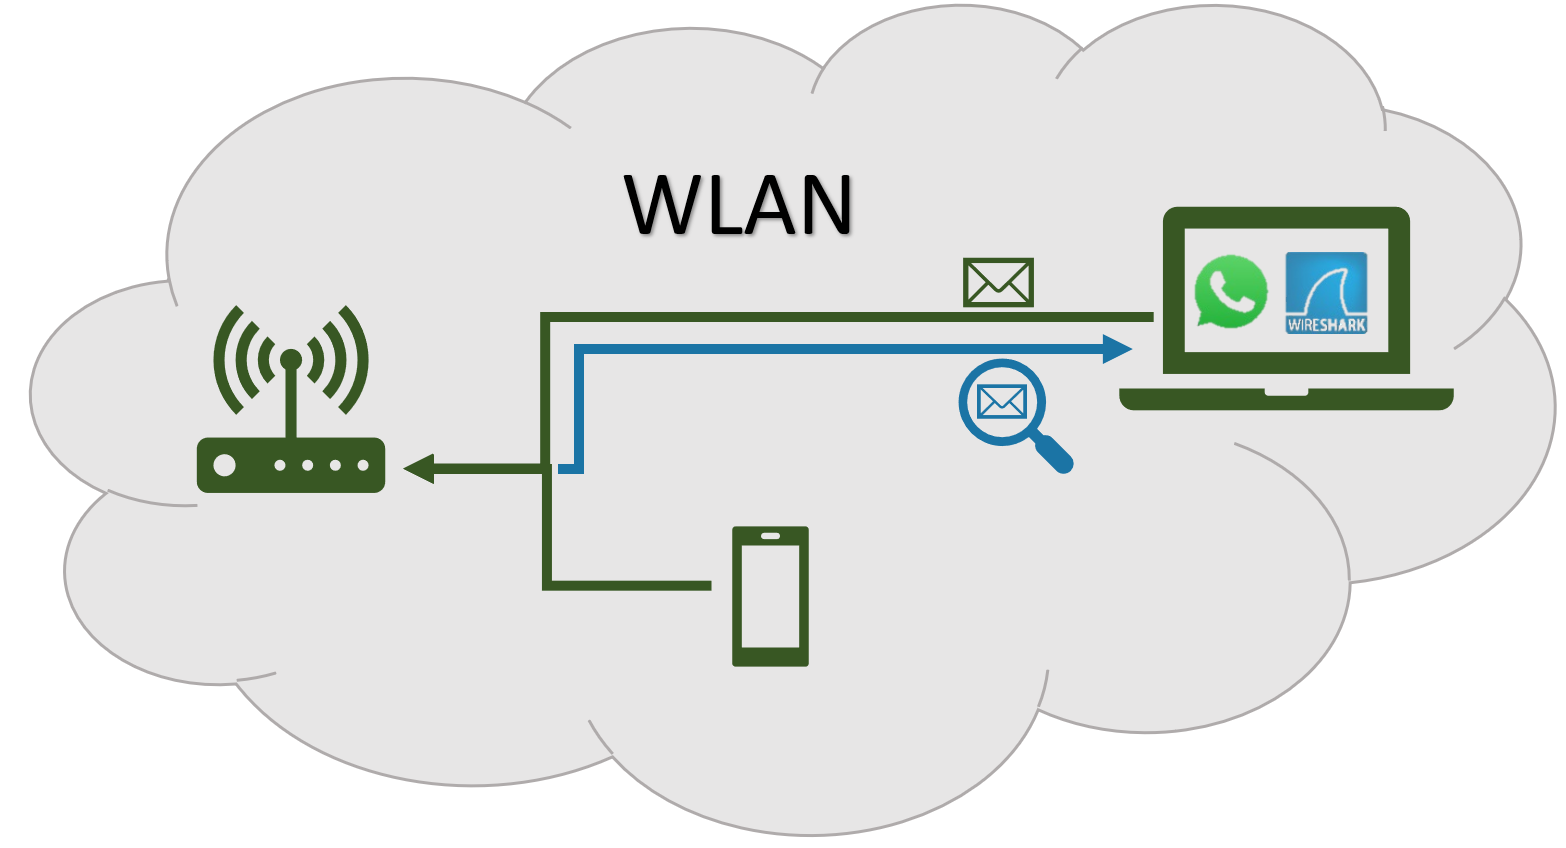
\includegraphics[width=9cm]{Aufbau}
\end{center}

\begin{description}
    \item \textbf{Laptop}
        \begin{description}
            \item \textit{WebWhatsApp}: 
                Über diesen Laptop wird WebWhatsApp aufgerufen. Der Client ist 
                bereits auf registriert. 
            \item \textit{Wireshark}:
                Zusätzlich ist Wireshark installiert um die gesamte Netzwerkkommunikation
                zu analysieren.
        \end{description}
    \item \textbf{Smartphone}
    \begin{description}
       \item Das Smartphone über das der Laptop Client bei WhatsApp registriert ist, muss
            sich im Internet befinden. In diesem Fall ist es im gleichen WLAN (müsste es aber nicht sein). 
    \end{description}
\end{description}

\subsection{Analyse mit Wireshark}
\subsubsection{Vorgehen und erster Überblick}
Da zunächst noch nicht bekannt ist, welche Pakete von WhatsApp verschickt werden.
Wird das Capturing von Wireshark ohne Capture Filter ausgeführt. Nachteil ist, 
dass dadurch viel zu viele Pakete angezeigt werden z.B. verschiedene Dropbox Jobs. 
Deshalb müssen zunächst die für die WhatsApp-Analyse relevanten Pakete bzw. Streams
gefunden werden. 
Die einfachste Möglichkeit ist es nach der IP-Adresse zu filtern. 
WebWhatsApp verwendet IPv6 und hat die Adresse: \texttt{2a03:2880:f22d:c5:face:b99c:0:167}. 
Mit diesem Display-Filter ist es möglich das 'Client Hello' Paket vom TLS.v3-Handshake zu finden. 

\begin{center}
    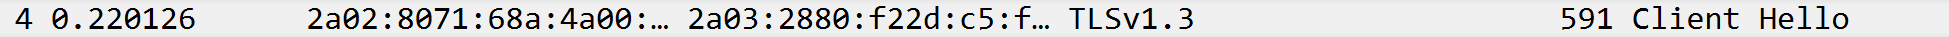
\includegraphics[width=14cm]{ClientHelloTLS}
\end{center}
Dieser SSL-Session kann im Anschluss gefolgt werden. So wird der gesamte SSL-Stream angezeigt.

\begin{center}
    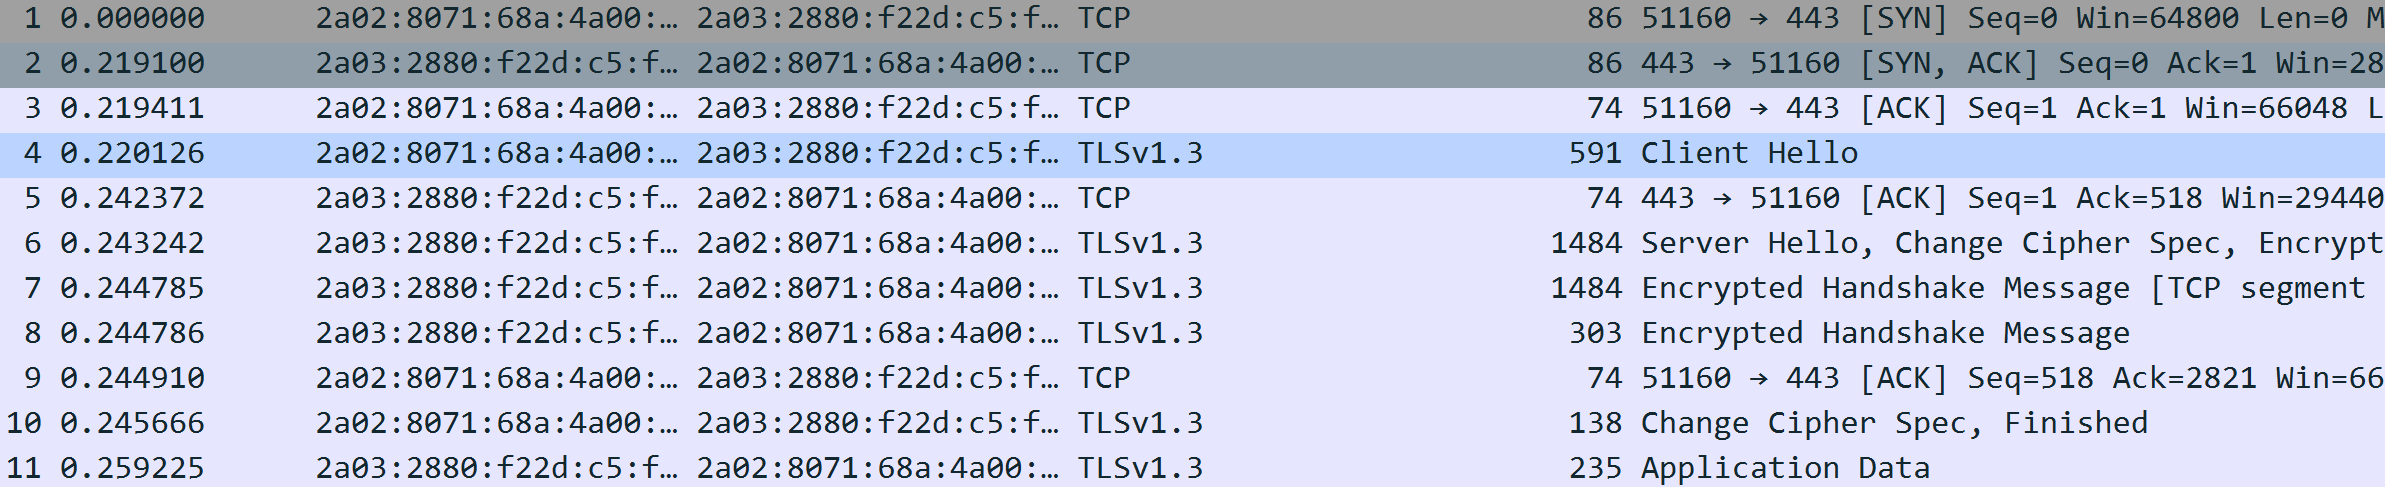
\includegraphics[width=15cm]{WhatsAppFilteredOverview}
\end{center}

In diesem Wireshark-Ausschnitt sind 4 Aktionen sichtbar:
\begin{enumerate}
    \item TCP Handshake
    \item TLSv1.3 Handshake
    \item TLS Cipher-Suite Einigung
    \item Übertragung der Daten von WhatsApp    
\end{enumerate}

Diese einzelnen Aktionen, die notwendig zum Aufbau der Session sind, 
werden im Folgenden genauer analysiert.

\subsubsection{TCP Handshake}
Die ersten drei Pakete des Wireshark-Snippets stellen den TPC Handshake dar.

\begin{center}
    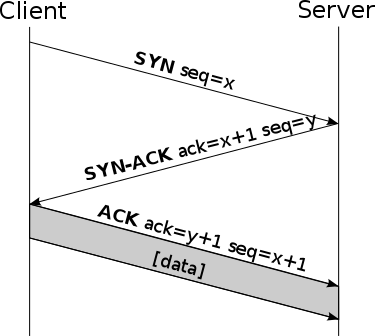
\includegraphics[width=4.5cm]{TCPHandshake0}
\end{center}
Dieser Handshake ist notwendig um eine Verbindung zwischen den beiden Sockets von Client
und Server herzustellen.

\begin{center}
    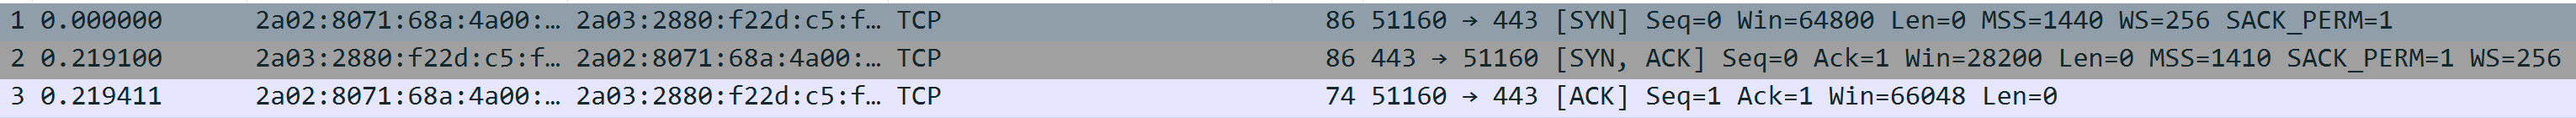
\includegraphics[width=15cm]{TLSHandshake1}
\end{center}
In diesem Wireshark-Snippet ist genau dieser Ablauf zu erkennen.
Wireshark bietet die Möglichkeit, die Pakete in einem Flowchart anzuzeigen. 
Dieser ist für einen Überblick sehr hilfreich.
\begin{center}
    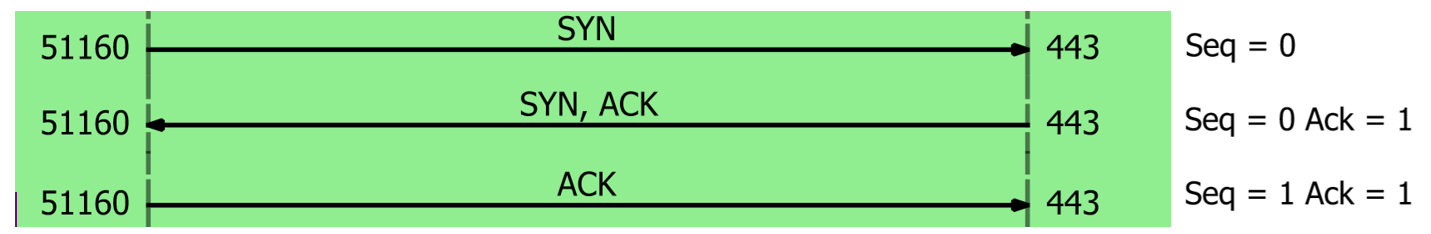
\includegraphics[width=10cm]{TCPHandshakeOverview} 
\end{center}

Zunächst sendet der Laptop (mit WebWhatsApp) das \texttt{SYN-Paket} mit einer Sequenznummer.

\begin{center}
    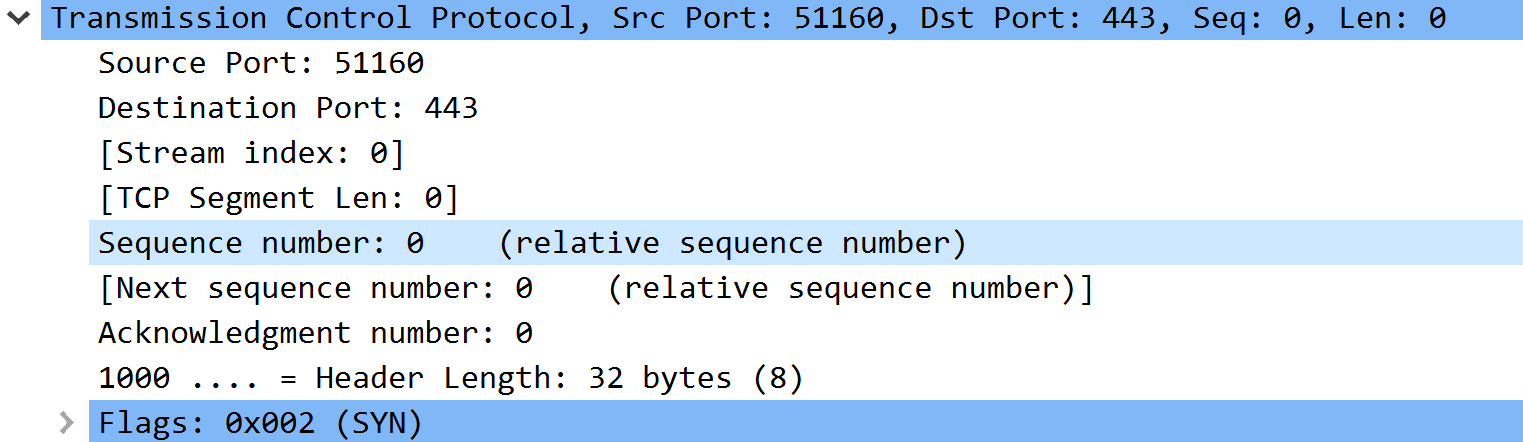
\includegraphics[width=10cm]{TCPHandshake1}
\end{center}

In diesem Fall ist die \texttt{Sequenznummer = 0}
Der Server antwortet mit einem \texttt{SYN-ACK-Paket}.

\begin{center}
    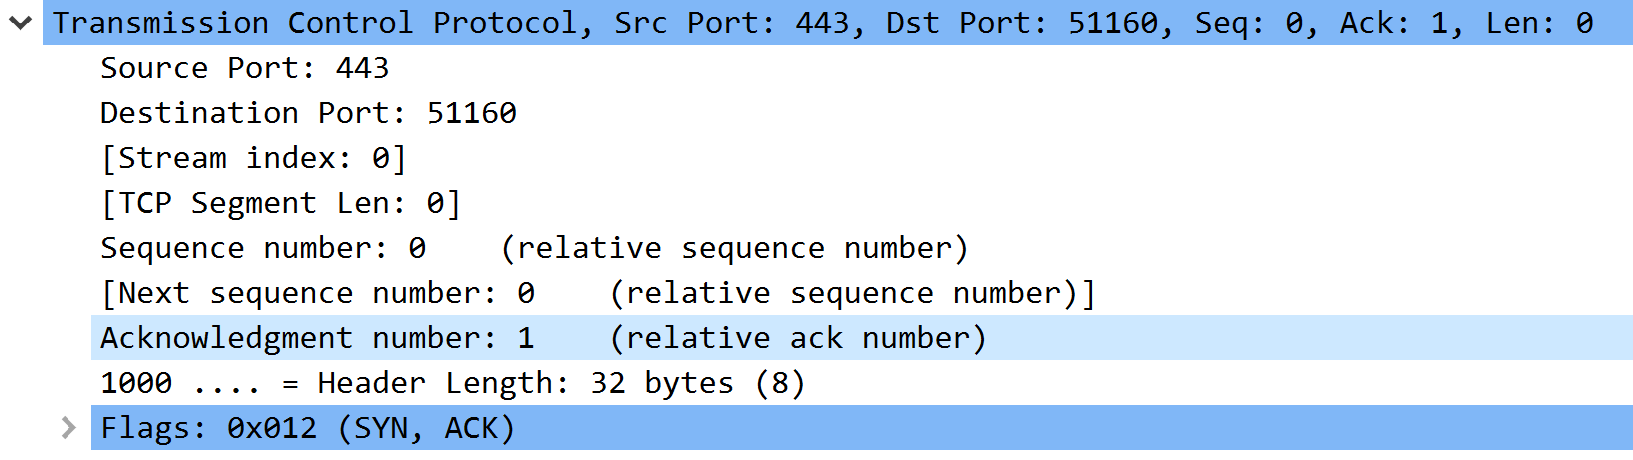
\includegraphics[width=10cm]{TCPHandshake2}
\end{center}

Dort ist die \texttt{Acknowledgementnummer = 1} und eine neue \texttt{Sequenznummer = 0}. 
Zum Abschluss des Handshakes sendet der Client dem Server seinerseits ein \texttt{ACK-Packet}.

\begin{center}
    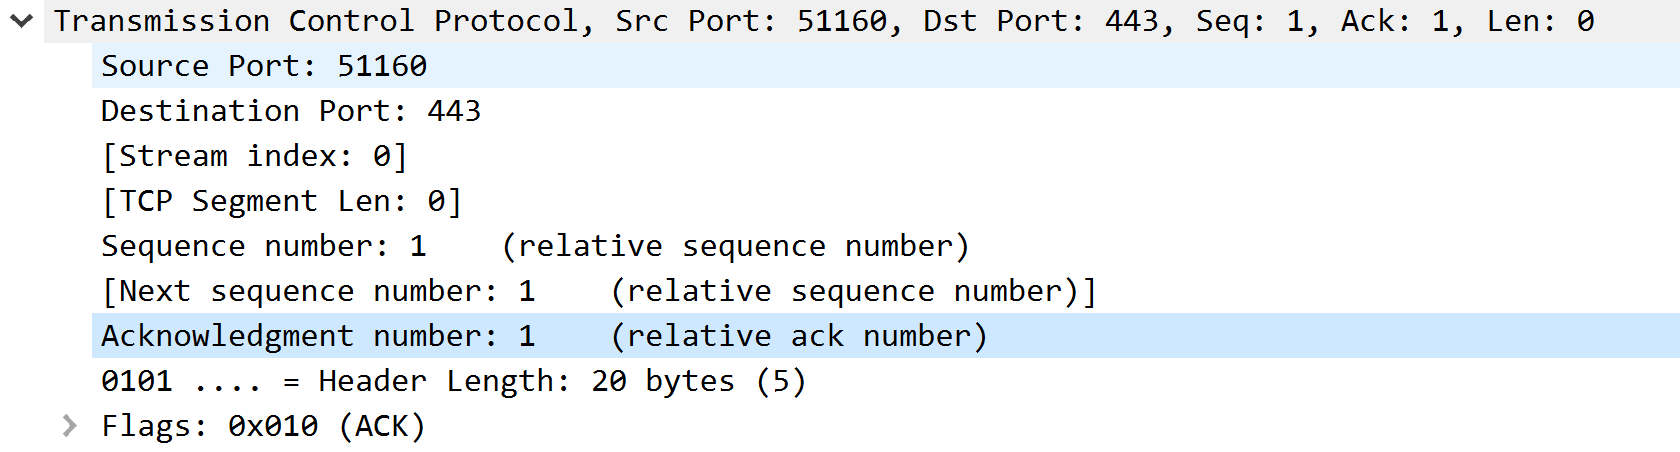
\includegraphics[width=10cm]{TCPHandshake3}
\end{center}

\subsubsection{TLSv1.3 Handshake}
Für den TLSv1.3 Handshake sieht der Flowchart der von Wireshark generiert
wird wie folgt aus.

\begin{center}
    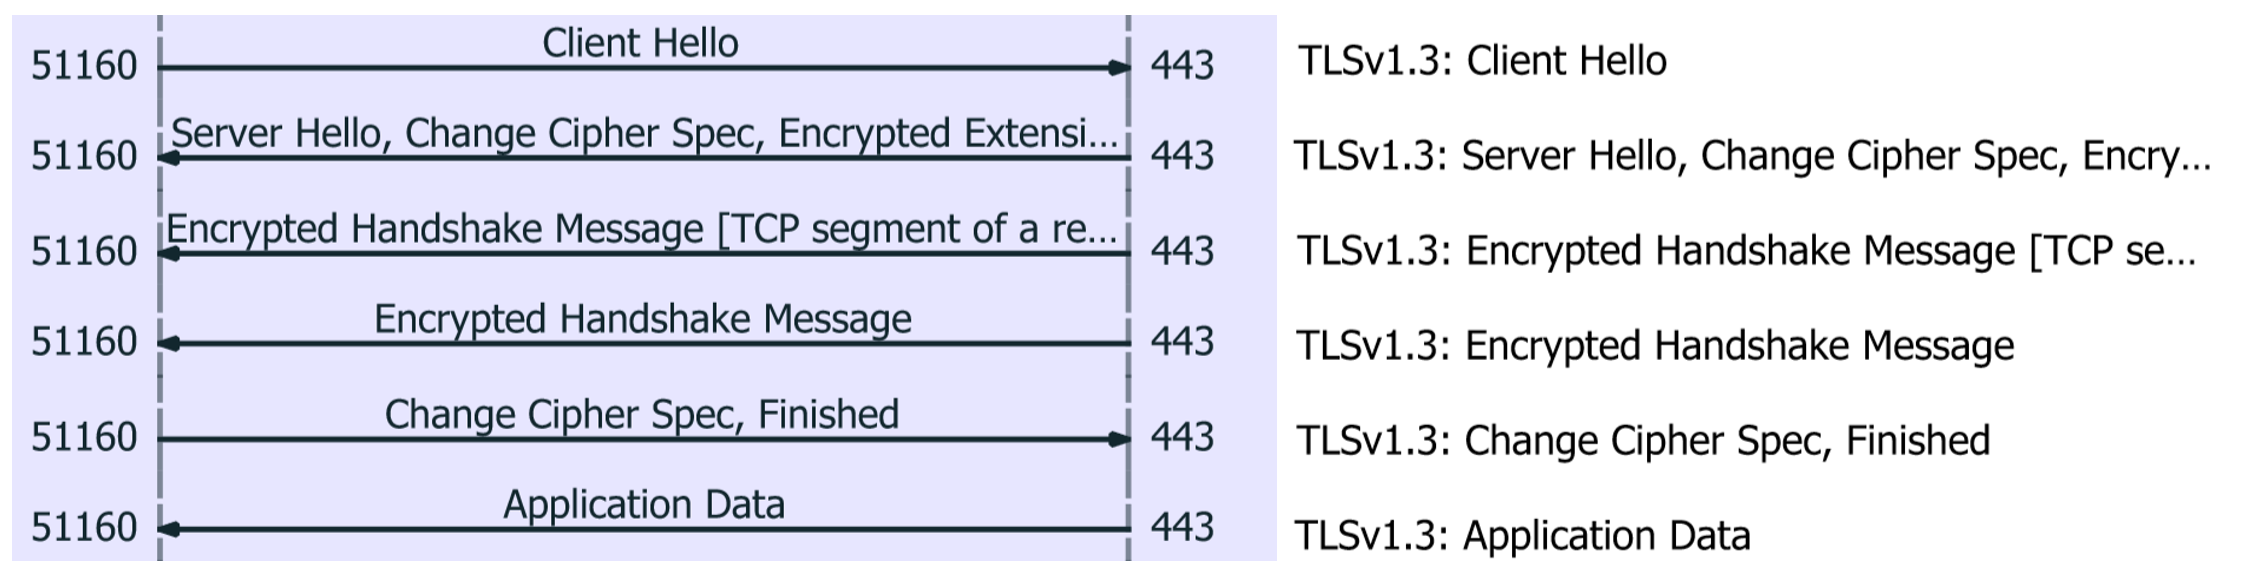
\includegraphics[width=10cm]{TLSHandshakeOverview}
\end{center}

\textbf{Client Hello}\\

\textbf{Sever Hello, Cipher Suite}\\

\textbf{Encrypted Handshake Message}\\

\textbf{Finished}\\

\textbf{Application Data}\\

\subsubsection{Einigen auf Cipher-Suite}
\subsubsection{Übertragung der Application Data}